\documentclass[12pt]{article}
\usepackage[margin=1in]{geometry}
\usepackage{graphicx}
\usepackage{times}
\usepackage[T1]{fontenc}
\usepackage{textcomp}
\usepackage{titlesec}
\usepackage{array, booktabs}
\newcommand{\sectionbreak}{\clearpage}

\graphicspath{ {img/} }

\begin{document}

\begin{titlepage}
  \begin{center}
    \vspace*{1cm}
    \Huge{\textbf{
        UAV Collision Avoidance\\
        Final Report
    }}

    \vspace*{1.5cm}

    \begin{figure}[ht!]
      \centering
      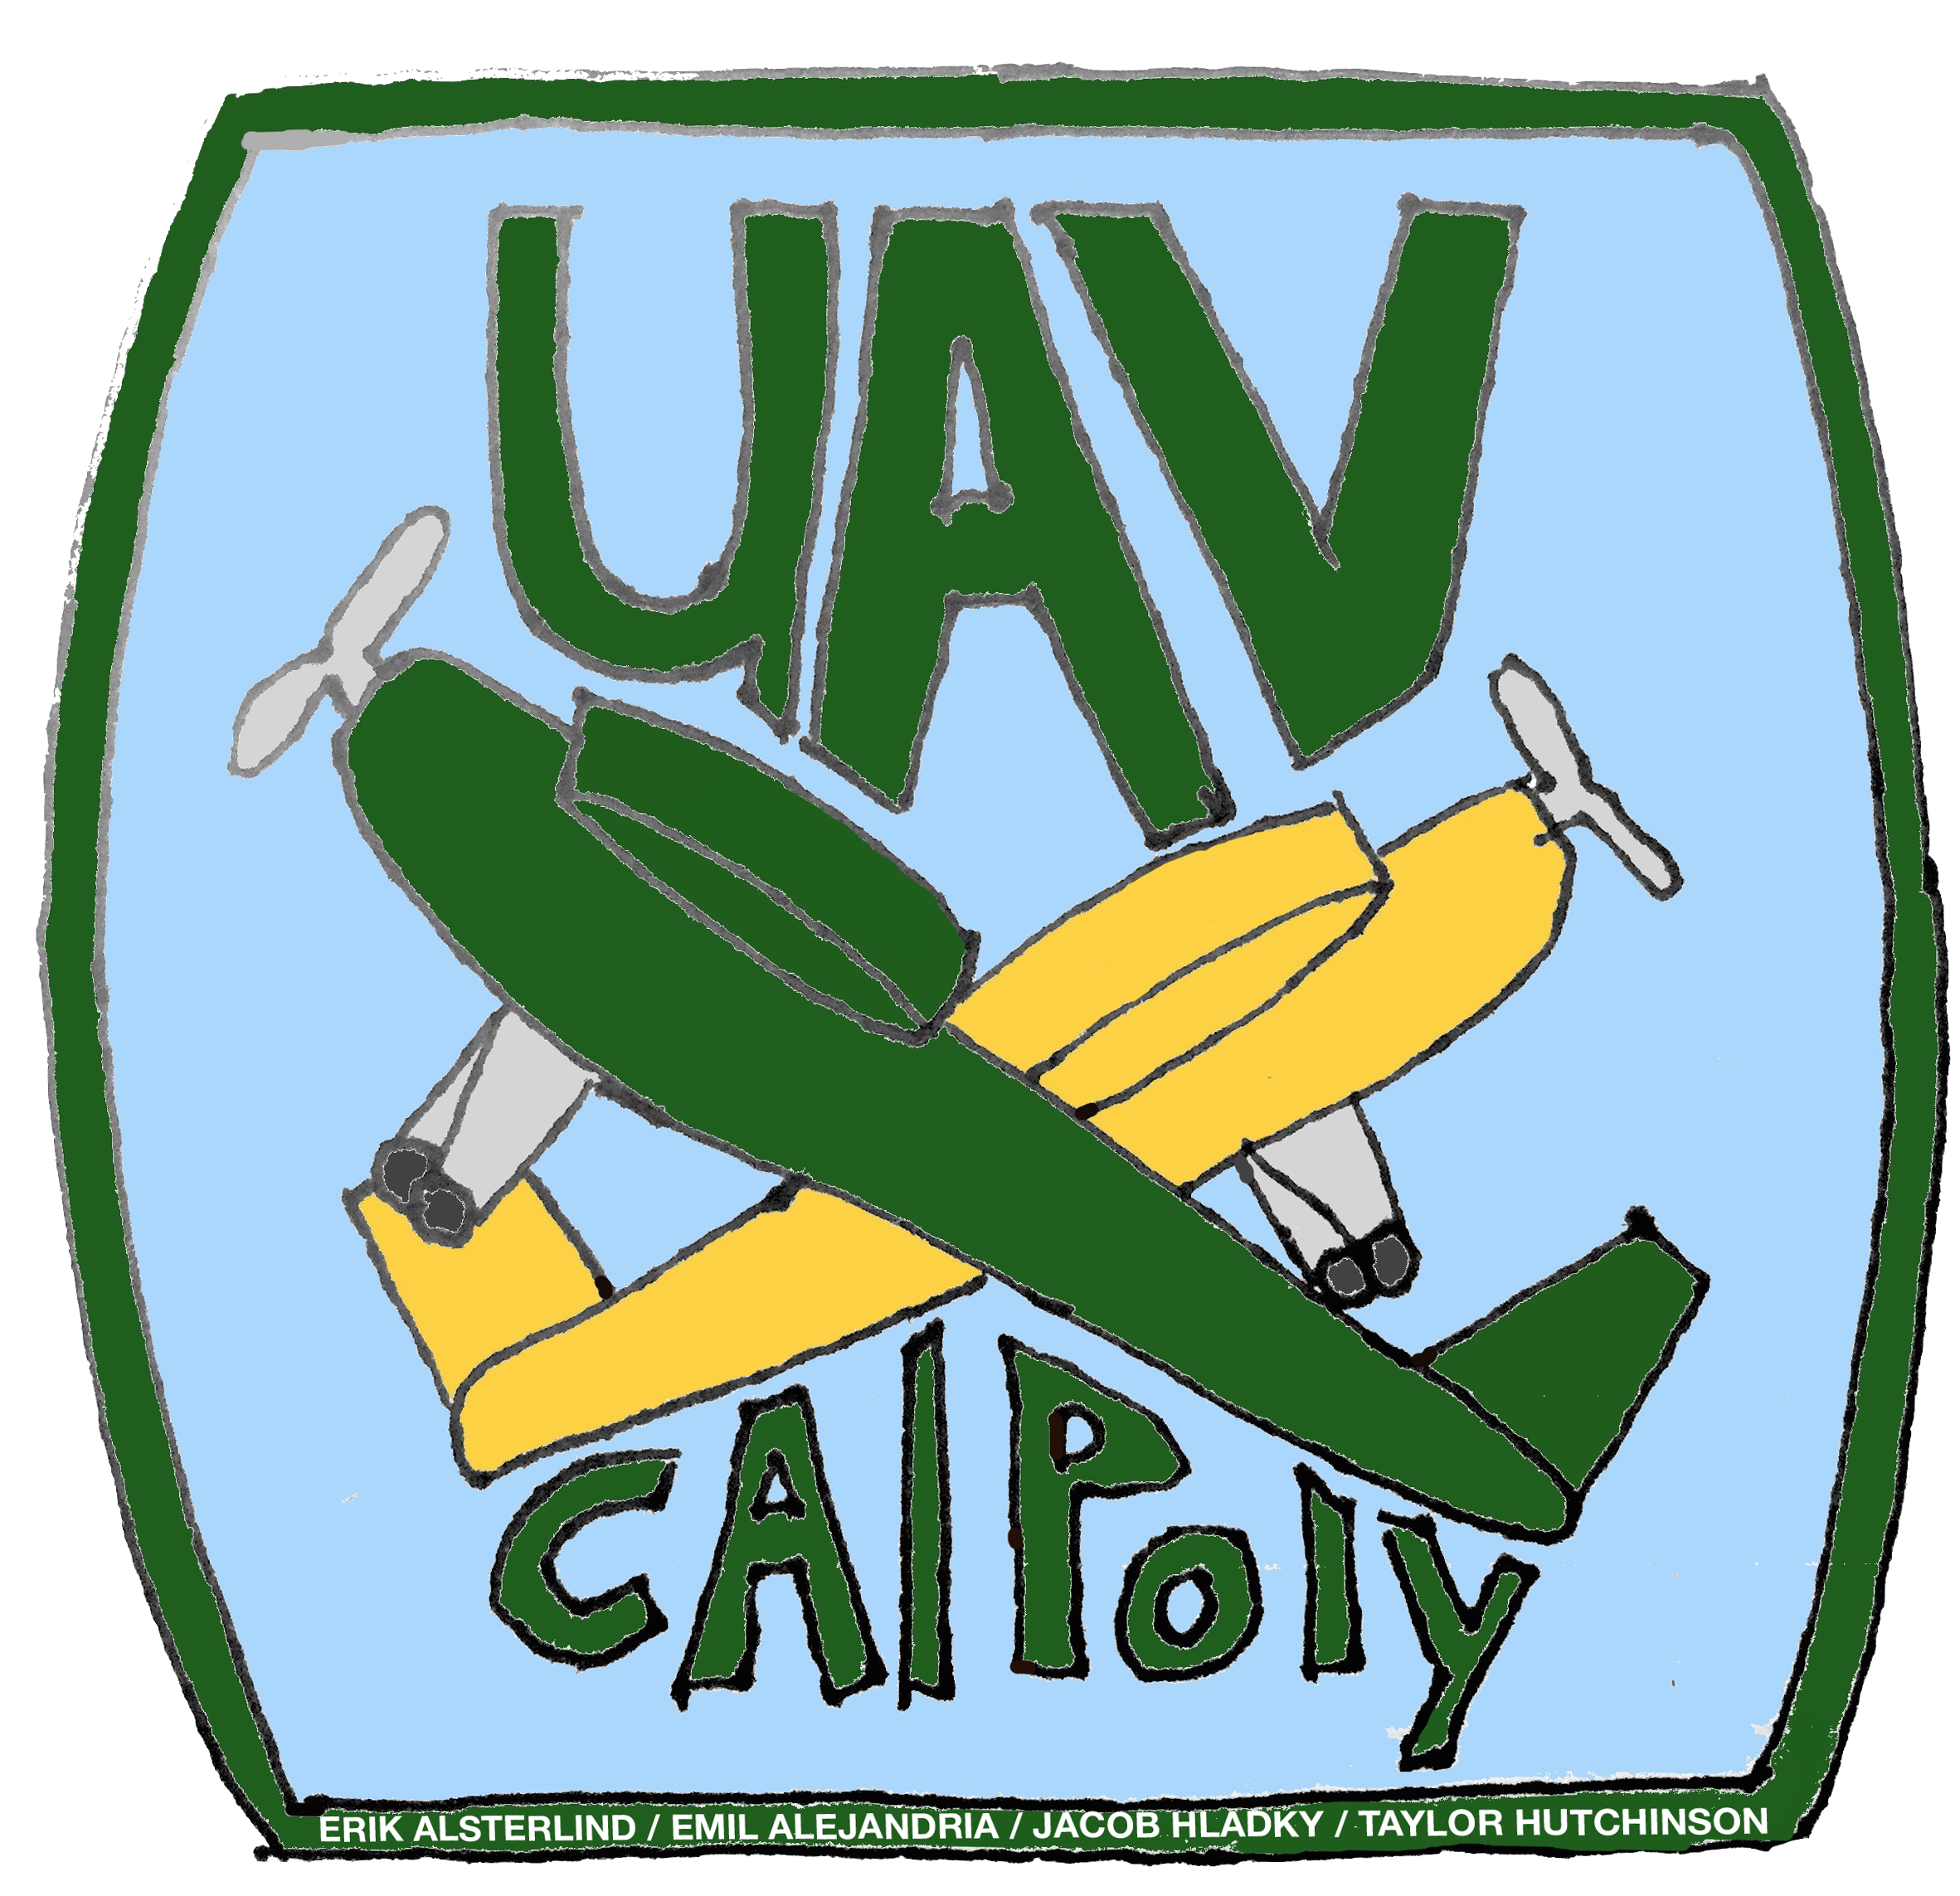
\includegraphics[width=0.5\textwidth]{logo.png}
    \end{figure}

    \vfill
    \large{
      Emil Alejandria\\
      Erik Alsterlind\\
      Jacob Hladky\\
    }

    \vspace{1cm}

    \large{
      Department of Computer Engineering\\
      California Polytechnic State University, San Luis Obispo\\
      \today
    }

  \end{center}
\end{titlepage}

\pagenumbering{roman}

\tableofcontents
\clearpage

\pagenumbering{arabic}

\section{Introduction}
\subsection{Project Overview}
The Northrup Grumman UAV project, started three years ago, is a collaborative effort between Cal Poly, San Luis Obispo and Cal Poly, Pomona. This collaboration has resulted in several autonomous vehicles, including several planes, a ground vehicle, and, most recently, a quad-copter. Last year the focus of the project was the implementation of a basic collision avoidance algorithm for the planes. This year, the focus was on maintenance, compatibility, and documentation. Specifically, the goals of this team were to upgrade the autopilot system and to improve the existing collision avoidance algorithm.\\\\
The result of this project was a more robust and extensible flight-controller, a more intelligent sense-and-avoid system, and a more accessible code-base.

\subsection{Clients and Community Partners}
Our client on this project is The Northrup-Grumman Corporation (NGC), one of the largest defense companies in the world, and one of the primary contractors for the United States Armed Forces. NGC benefits from continued collaboration with Cal Poly and Cal Poly, Pomona as the universities provide the company a ready supply of talent for potential hire after graduation as well as a possible source for innovation.\\\\
Students benefit from NGC’s involvement by exposure to the corporate requirements and practices of large, multi-disciplinary projects, and by the opportunity to work on complex hardware systems.

% NOTE, THIS SHOULD BE MOVED TO SOME OTHER SECTION.
% The final outcome of project is some years down the road, but it will include a UAV with a sophisticated autopilot capable of understanding and reacting input to several sensors, including a GPS receiver, a radio link to a base station and a partner UAV. Our project deliverable is a small section of the overall goal: a well written collision avoidance heuristic, and a framework to verify its correctness.

\subsection{Stakeholders}
The stakeholders most immediately affected by our work on the UAV are the other members of the project that are outside of the Capstone group. How the system operates reflects on every member of the team regardless of what each member actually worked on. If everyone in the team does a great job on their own responsibilities, everyone will benefit when the demonstration takes place at the end of the year.\\\\
The Cal Poly Pomona team, working on their own version of the UAV system, has a significant stake in the outcome of our group’s project. They had previously attempted to build a collision avoidance system but it was non-functional. If successful, our system would both lead to a more successful mutual demo, reflecting well on both teams, and also give us the knowledge to potentially help the Pomona team with any residual issues they might be having. Additionally, both Cal Poly Pomona and Cal Poly SLO universities are stakeholders in this project. This project provides a valuable resource to help students at the schools pursue their interests and forward their career prospects.  Also, the schools can potentially use projects like ours that involve high profile sponsors as recruitment tools for future students.\\\\
Finally, there are external stakeholders that might have to rely on our system to perform their job. These potential stakeholders include the military, search and rescue teams and companies in need of a delivery system such as Amazon. In the case of the military and search and rescue teams, the performance of the UAV could mean saving or losing lives which makes the effectiveness of our system critical. In the case of a company like Amazon the use of UAVs to deliver products may not put any lives at risk, but its still a significant economic investment for a company to make. If our system does not perform than that means a loss in terms of money invested as well as customers that aren’t serviced adequately.

\subsection{Framed Insights and Opportunities}
In our initial meeting with Northrop representatives they explained that they expect a polished mid year presentation and look at this project as a recruitment opportunity. Northrop is sponsoring this project and they expect a professional and well thought out presentation to communicate our design, which will give them a clear image of what their time and money is producing. Additionally, as a large company they are in constant need of new talent to add to their workforce. If we can do a great job on this project than that gives Northrop an immediate pool of talent to draw from that they know is up to their standards.\\\\
A group of stakeholders that have needs separate from the client is the non-Capstone members of the UAV team. They need us to do a good job on our part of the project and be available to communicate about the project as necessary. The first point is important because how well we execute our part of the project will reflect on every member of the group. Additionally, the team needs us to be effective communicators to avoid issues between different branches of the project. For example, if we need a sensor mounted on the aircraft we need to let the right people know promptly so they can execute our request in a manner that makes sense for them. If we don't adequately describe what we want, or don't let them know till the last minute, issues can easily arise.\\\\
With respect to the more external stakeholders, the only need is for our system to function. We likely will never speak directly to any member of the military or search and rescue team, but they will only employ our system if it functions as expected. If a UAV loaded with our logic and hardware system is sent out to deliver supplies or locate a lost person, than that is exactly what the system needs to do. It is up to us to make sure our design is implemented effectively to meet these potential needs that could have massive real world ramifications.\\\\

\subsection{Goals and Objectives}
Goals:
\begin{enumerate}
\item Redesign the existing GPS based collision avoidance system to operate more effectively and reliably.

\item Develop a sense and avoidance system for a UAV that is capable of functioning in a GPS denied environment.
\item Design a simulation suite to emulate the real world environment that the planes will be operating in.
\item Emphasize the documentation and organization of the project to aid future capstone teams in improving the project.
\end{enumerate}
Objectives:
\begin{enumerate}
\item Understand the technical capabilities, requirements, and limitations of all potential platforms available to us so that we can select the optimal platform for our needs.
\item Draw a complete picture of environmental variables necessary to design a simulator that can sufficiently emulate a field test.
\item Outline the shortcomings in the project's documentation and work to make documentation a strength of the project rather than a weakness.
\end{enumerate}

\subsection{Outcomes and Deliverables}
By the end of our term on the project we will have completed a sense and avoid system that is capable of operating in both a GPS enabled and GPS denied environment. The system will take an initial GPS coordinate and using sensors to track movement, update its position and be able to transmit it to nearby UAVs. Upon recognizing an imminent collision it should react according to the situation without preventing it from reaching its target. Beyond this, we hope to have left tools for future teams of capstone students to use as they pick up and develop this project.\\\\
The stewardship we intend to bring to the project should allow them to pick up where we and previous teams have left off with ease and the simulation software should speed up the development process of future systems that they plan to implement. Any of the code worked on should be professionally commented; system improvements, revisions, and issues should be well documented, and the simulation software should be dynamic and easy to use with a user manual.

\section{Background}
At the end of the project's previous year, the team was able to successfully demonstrate a functioning sense and avoidance system. However, this system was dependent on an accurate and reliable GPS signal and in need of substantial hardware improvements.\\\\
The new system will utilize a variety of sensors to alleviate the dependence on GPS and still maintain an accurate location. The potential sensors desired include inertial measurement units, infrared sensors, optical sensors, and small-scale radars. A number of solutions exist online concerning inertial navigation systems, however many of them suffer from either being too expensive or wildly inaccurate after short durations.[1] Infrared sensors typically lack the range to be useful in our application[2], optical sensors require computing power that may be beyond the capability of our hardware[2], and radar systems tend to consume excessive amounts of power.[2] Individually any of these sensors are grossly inadequate but combining sensors has been shown to provide remarkable improvements in navigation system reliability, such as a simultaneous localization and planning (SLAM).[3][4] However, for such systems it has been posited that Kalman filters provide an inadequate solution due to the dependence on inertial sensors and that alternative solutions must be sought.[3]\\\\
The previous hardware posed cumbersome limitations on the avoidance system as it was barely capable of processing all the required tasks. The new system will use a 3D Robotics Pixhawk for all computational needs. The only exceptions are the wireless communications and potentially another unit for sensor input processing. The Pomona team has previously used a Pixhawk in their system with arguable success, but advised against their usage despite the theoretical gains because it did not meet their technical specifications. The code will also be reimplemented in a lower level manner to help improve efficiency. A number of autopilot systems are available that provide general libraries, however such accommodation comes at the cost of efficiency.[5] However, the issue of collision avoidance in UAVs is well-researched area and documentation is in abundance to help design a solution specific to our particular needs.[6]

\section{Engineering Specifications}
\subsection{Goals}
Our goals are to build a working implementation of military UAV technologies. We will redesign and implement a collision avoidance algorithm for the UAV. To make this possible we will also upgrade the hardware in the UAV. We will develop a test environment to effectively diagnose the system on the ground and to help future groups develop new software for the UAV.

\subsection{Specifications}
Discussion of high risk requirements is located in the requirements table.

\subsubsection{Minimum Detection Radius}
This specifies the minimum distance the UAV must be from another UAV or object when it enters collision detection mode. This specification is critical because it corresponds with the turning radius of the UAV and the time the algorithm takes to determine  what to do. If the algorithm detects a collision at a distance less than specified, an actual collision may occur because there is not enough time or space to avoid the object.

\subsubsection{Collision Recovery Time}
After entering and exiting collision detection mode, several cleanup operations may need to occur. In and airspace that contains another vehicle in flight, the UAV may need to enter collision avoidance mode repeatedly. Thus the amount of time to reset the collision detection algorithm is of a high risk.

\subsubsection{Fall Back to Manual Control}
If the algorithm malfunctions, it may be necessary to land the UAV to avoid a crash. Thus it is absolutely crucial that the autopilot can be disengaged at any time.

\subsubsection{Collision Detection Delay}
This specification determines how quickly the algorithm evaluates whether it should be in collision detection mode. It is important in complicated environments where the UAV may encounter an object it needs to avoid, and then encounter another object in the process of avoiding the first. In this complicated case the UAV needs to accurately assess what to do and not, for example, turn back into the original object. This specification is distinct from the recovery time specification because it deals with the complicated behavior within the algorithm from a white-box perspective, whereas 3.2.2 is a black box specification.

\subsection{Requirements Table}
Herp Derp

\section{Final Design Overview}
\subsection{The Final Design}
The centerpiece of the hardware setup we instituted is the 3D Robotics Pixhawk with PX4 autopilot system. This unit contains a 32 bit ARM processor running at 168 MHz and the NuttX Real Time Operating System. This system is replacing the combination of Ardupilot Mega and APM 2.6 microcontrollers that were the brains of the previous iteration of this project. The updated hardware system architecture can be seen below in Figure 1.

<Figure 1>

The increased wordsize of the Pixhawk along with its significantly faster clock rate provides our new system with a much more powerful brain to perform computations and manage modules. We used 3D Robotics GPS modules that came with the Pixhawk to provide GPS points for our sense and avoid algorithm, which plugged into a designated port in the module.\\\\
The other hardware component we integrated is the Digi International Xbee S3B Pro radio module for communication between UAVs. The Xbee is connected to the Pixhawk via UART serial connection, of which the Pixhawk has three open ports for use. Hardware wise, this connection is relatively simple. The 5 Volt pin of the Pixhawk port goes through a voltage regulator which brings it down to 3.3 Volts for the Xbee power pin. The TX and RX pins of both modules are crossed (TX of Pixhawk port to RX of Xbee and vice versa), and the ground pins are connected. In terms of software, the operation of the Xbees is performed through three functions. The first function opens and configures the UART Port of the Pixhawk through software. In our code this function is called “uart\_init()”, and can be reviewed in our software documentation which is listed in the appendix of this report. After initialization, we have a function that writes a buffer of data to the xbee, and a function that reads a specific number of bytes of data from the Xbee into a buffer. Both functions, \texttt{xbee\_send()} and \texttt{xbee\_recv()}, can be viewed in the aforementioned software documentation. In Figure 2 below you can see a software flow diagram of how the uses of the Xbee are integrated into the software of the system using these functions.\\\\
The sense and avoidance algorithm uses a potential field method to generate a path to the goal. The algorithm works off of the idea of potential fields, emulating the forces found in nature such as magnetism and gravity. Every known entity generates a potential field of vectors either pointing towards or away from itself. Obstacles generate vectors that push away from themselves and objectives generate vectors that pull towards themselves. The algorithm uses these vectors to find an efficient path of least resistance to the goal. A demonstration of this algorithm can be seen in fig. 3 below. The magnitude of the vectors are scaled with the distance to the obstacle. As the distance to the obstacle, the magnitude of the vectors rises exponentially. The exponential heuristic encourages minimal deviations from the straight path, but allows for a safe buffer zone between planes.

\subsection{Safety Concerns}
With respect to safety, the primary concern with our system is the safety of the planes in flight, and any bystanders that might be viewing our demonstration. To make sure both the mechanical and biological systems involved stay safe and intact we will be employing our own test environment to put our algorithm through its paces. We will be building this environment in parallel with the construction of the UAV to make sure we can test our code thoroughly before anything is put in the air. The goal is to test our algorithm until we know it will function as intended every single time. This way, we can ensure the planes stay on course in the air, and there is little to no risk of a crash. The test environment will be step based, which means iterations will come in small intervals of time to emulate the processing of the planes in the air. Additionally, data from test flights will be replicated and fed into the algorithm to make the tests as realistic and relevant as possible.

\subsection{Project Cost}

\section{System Integration and Testing}
\subsection{FMEA}
Our FMEA Identified 3 major points of failure, each with a few specific ways it could fail. Those points of failure are:
\begin{enumerate}
\item UAV Platform - the hardware keeping the UAV in the air fails in some way. Methods of failure:
  \begin{itemize}
  \item Loss of control
  \item Engine failure
  \item Loss of power
  \end{itemize}
These failures are addressed by the platform team within the UAV group.
\item Pixhawk Failure - software or hardware problems related to the pixhawk. Methods of failure:
  \begin{itemize}
  \item Algorithm failure
  \item Hardware failure
  \end{itemize}
Algorithm failure means that we located an obstacle, but failed to avoid it. Hardware failure, on the other hand, would be electric failure of the pixhawk processor.
\item XBee Failure - the communication is interrupted or invalidated somehow. Methods of failure:
  \begin{itemize}
  \item Loss of connection
  \item Bad data
  \end{itemize}
\end{enumerate}
%These and other possible failures are all addressed in our risk management document located on dropbox at “RMAX Helicopter Project\\Cal Poly Capstone 2014\\Processes for Handling Risks.docx.”

\subsection{DVP+R}
The following tests were explored in our DVP+R:
Pixhawk Resilience Test: subjecting the pixhawk to physical stress similar to what it would endure while in flight to ensure integrity.
Object Detection Test: place multiple objects / planes in the environment and ensure that the system identifies all of them.
Beacon Test: Place GPS beacons in the flight area and ensure that the system avoids them.
Waypoint Test: Have plane navigate through an environment with obstacles and ensure it arrives within 10m of waypoint.
Connection Verification Test: Send packets via XBee in potentially lossful environments (different planes, different orientations, etc) and ensure data arrives.
Packet Verification Test: Send packets via XBee in potentially lossful environments and ensure data validity.
IMU Test: Move the hardware while the IMU is running to test for accuracy

There were a few more tests we explored, but they did not apply directly to us, rather to the platform team in regards to ensuring the platform is sound. They can be found in the DVP+R Section of the appendix.

\subsection{Overall System Analysis}
\subsubsection{Collision Avoidance Algorithm}
%In regards to our collision avoidance (sense & avoid) algorithm, we have met all requirements as can be verified without flying the planes. Unfortunately, due to FAA and CSU regulations, we are unable to fly at this time and as such cannot be 100% certain our algorithm works. See the requirements table in section 3.3 for the full list.  Notable requirements met:
Minimum Detection Time
Minimum Buffer Zone
Maximum Algorithm Run Time
Object Detection Radius

\subsubsection{Simulation Environment}
At this time, we have been unable to begin work on the simulation environment. See future plans (5.4) for more information.

\subsubsection{Code Stewardship}
We are continuing to improve our code stewardship, and have met all requirements as in the table in section 3.3. We have also placed all our code on a github repository for easy access and management. The private repo is provided to us by the IEEE club, and is the “Cal Poly IEEE/firmware” repository.

\subsubsection{Future Plans}
%	The UAV project is one that has been going on for over 3 years, and we still have quite a few plans in store. In regards to the sense & avoid algorithm, there is still much improvement to be made. We are working on adding additional components to our vectors orthogonal to the heading of incoming planes to more accurately avoid them without being pushed away from our destination. We are also working on adding more factors to the calculation of these vectors, such as plane velocity and heading.
	At this point, the simulation environment is still planned, but has not yet been started. The capstone team was unfortunately too busy to address it. This will be a major undertaking, and will require many sets of flight data to validate it. Since the project is grounded right now, acquiring these logs is somewhat troublesome. Once they are available, development can begin in earnest.
	Another important part of the future of this project is the hardware. Since we have just upgraded to the pixhawk, there are a lot of clock cycles we have to work with. The future of the hardware development will be sensors. The first sensor that will be added is a camera for computer vision. This may also include a separate board to interface with the camera via firewire and handle the calculations. More sensors may be addressed in the future.

\section{Management Plan}
\subsubsection{Team Mission and Team Objectives}
%	Our team mission was to upgrade the on-board hardware and the sense & avoid algorithm while making the whole project easier for new members to approach. Our first objective was to upgrade the autopilot hardware by purchasing & integrating the pixhawk PX4 autopilot. Our second objective was to upgrade the sense & avoid algorithm, which we did by implementing the modified potential field algorithm. Our final objective was to make the project more approachable, which we did be creating thorough code documentation and better instructions for setting everything up. This objective was also helped by the pixhawk's expansive online resources.

\subsubsection{Team Membership and Roles}
Emil Alejandria                 	Team Lead, Sense and Avoid Architect
Erik Alsterlind                   	Quality control, System architect
Taylor Hutchinson           	Software architect, Sense and Avoid Architect
Jacob Hladky                    	Development tools specialist, procurement

\subsubsection{Development Schedule}

<Uhh>

	We spent around 6 hrs/person/week on this project. It should also be considered that while it may seem like we could have accomplished more in that time, a large amount of time went into preparing for presentations, especially the NGC design review on 3/6/15. The collision avoidance development spans a long time because while we had a working algorithm in a couple weeks, we are constantly looking for ways to upgrade and improve it.

\section{References}
\begin{enumerate}
\item Kim, Jong-Hyuk, Salah Sukkarieh, and Stuart Wishart. ``Real-Time Navigation, Guidance, and Control of a UAV Using Low-Cost Sensors.'' Field and Service Robotics (vol. \# 24). New York: Springer-Verlag Berlin/Heidelberg, 2006. N. pag. Print.
\item ``UAV Sensors -- Electro Optical, Infrared and SAR.'' UAV Sensors -- Electro Infrared and SAR. N.p., n.d. Web. 14 Oct. 2014.
\item ``Passive GPS-Free Navigation for Small UAVs.'' Langelaan, J. Aerospace, 2005 IEEE Conference 5-12 March 2005,. Piscataway, NJ: IEEE, 2005. IEEE Xplore. Web. 13 Oct. 2014.
\item Kim, Johnhyuk, and Salah Sukkarieh. ``SLAM Aided GPS/INS Navigation in GPS Denied and Unknown Environments.'' Australian National University. Proc. of The 2004 International Symposium on GNSS/GPS, Australia, Sydney. CECS, n.d. Web. 13 Oct. 2014.
\item ``OpenPilot.org -- The Next Generation Open Source UAV Autopilot.''OpenPilotorg The Next Generation Open Source UAV Autopilot RSS. N.p., n.d. Web. 14 Oct. 2014.
\item Lacher, Andrew R. Unmanned Aircraft Collision Avoidance: Technology and Evaluation Methods (n.d.): n. pag. Www.mitre.org. Web. 13 Oct. 2014.
\end{enumerate}

\section{Appendix}
PDF's for the FMEA, DVP+R, Decision Matrix, Processes for Handling Risks, and Personas are all available in dropbox in the ``RMAX Helicopter Project/Cal Poly Capstone 2014'' folder. A compilation of all these documents can be found in the ``Final Report Appendix.pdf'' file.


\end{document}
